\documentclass{jsarticle}
\usepackage{listings,jvlisting} % 日本語のコメントアウトをする場合jvlistingが必要
\usepackage{color} % ソースコードの色塗り
\usepackage[dvipdfmx]{graphicx}
\usepackage{amsmath,amssymb} % 数式
\usepackage{here}

\usepackage[%
 dvipdfmx,% 欧文ではコメントアウトする
 setpagesize=false,%
 bookmarks=true,%
 bookmarksdepth=tocdepth,%
 bookmarksnumbered=true,%
 colorlinks=false,%
 pdftitle={},%
 pdfsubject={},%
 pdfauthor={},%
 pdfkeywords={}%
]{hyperref}

\usepackage{pxjahyper}

\lstset{
  basicstyle={\ttfamily},
  identifierstyle={\small},
  commentstyle={\smallitshape},
  keywordstyle={\small\bfseries},
  ndkeywordstyle={\small},
  stringstyle={\small\ttfamily},
  frame={tb},
  breaklines=true,
  columns=[l]{fullflexible},
  numbers=left,
  xrightmargin=0zw,
  xleftmargin=3zw,
  numberstyle={\scriptsize},
  stepnumber=1,
  numbersep=1zw,
  lineskip=-0.5ex
}

\begin{document}

\title{マルチエージェントシステム藤井先生レポート1}
\author{03-230966 河田顕帆}
\maketitle
\section{課題1}
私は、PSOのプログラムを作成して、6つの関数に対してPSOの性能を評価した。以下のサンプル数は幅10に対して100サンプル取るようにしている。また、次元数は2と20の2種類を試した。step数はいずれも500ステップである。\\
また、最適解との差は、2乗ノルムで計算した。\\
\begin{enumerate}
    \item Sphere関数 \\
        関数の係数等は以下の設定で行った。
        \begin{equation}
            f(x) = \sum_{i=1}^{n} x_i^2,  (-5.00 \leq x_i \leq 5.00)
        \end{equation}
        この場合、最小値は全次元0のxを与えた際の0である。\\
        以下に、次元数とサンプル数を変化させた際の結果を示す。グラフは、各ステップにおける最適解との差の対数をプロットしたものである。
        \begin {itemize}
            \item 次元数: 2, サンプル数: 100, ステップ数: 500 \\
                図から分かるようにステップを経るにつれて最適解との差の対数が単調にほぼ一様に小さくなっている。収束した様子は見られず、ステップ数を増加させれば収束した可能性がある。また、非常に最適値と近い値をとっていることがわかる。\\
                \begin{figure}[H]
                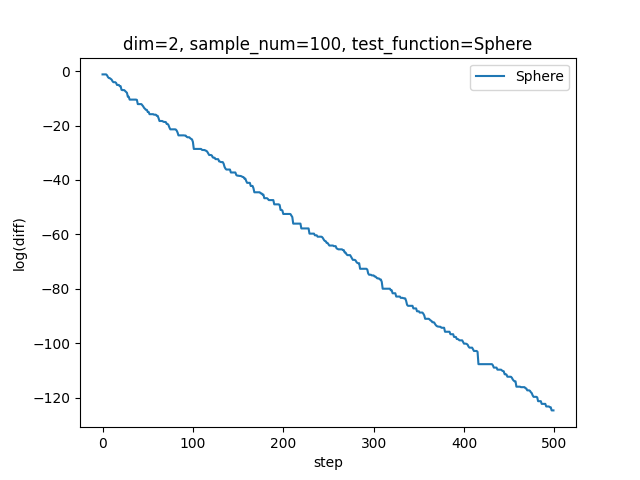
\includegraphics [width=10cm] {./result/Sphere_N_2.png}
                \end{figure}
            \item 次元数: 20, サンプル数: 100, ステップ数: 500 \\
                図から分かるようにステップを経るにつれて最適解との差の対数が小さくなっているが、次元数が2の場合のようにほぼ一様に減少するのではなく、50step程度までで急激に減少し、その後の減少は緩やかである。ここで収束したものと思われる。\\
                \begin{figure}[H]
                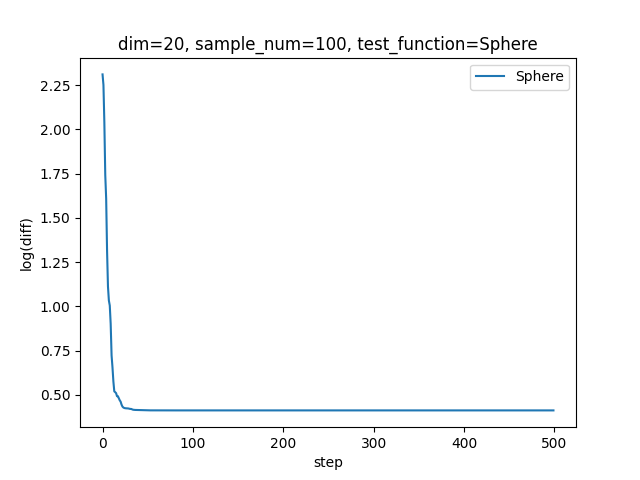
\includegraphics [width=10cm] {./result/Sphere_N_20.png}
                \end{figure}

        \end{itemize}
    \item Rastrigin関数
        関数の係数等は以下の設定で行った。
        \begin{equation}
            f(x) = 10n + \sum_{i=1}^{n} (x_i^2 - 10\cos(2\pi x_i)),  (-5.00 \leq x_i \leq 5.00)
        \end{equation}
        この場合、最小値は全次元0のxを与えた際の0である。\\
        以下に、次元数とサンプル数を変化させた際の結果を示す。グラフは、各ステップにおける最適解との差の対数をプロットしたものである。
        \begin {itemize}
            \item 次元数: 2, サンプル数: 100, ステップ数: 500 \\
                図から分かるようにステップを経るにつれて最適解との差が100ステップまでは単調に小さくなっているものの、そこで収束したと思われる。最適値との誤差は非常に小さな点で収束したことがわかる。\\
                \begin{figure}[H]
                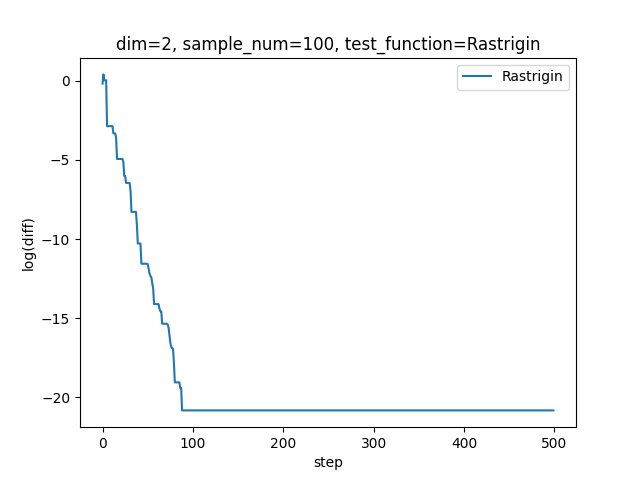
\includegraphics [width=10cm] {./result/Rastrigin_N_2.png}
                \end{figure}
            \item 次元数: 20, サンプル数: 100, ステップ数: 500 \\
                一度急速に最適値へと近づいたものの、再び誤差が大きくなってから収束したと思われる。各ステップでの変動幅が大きかったせいで最適値を通り越してしまって局所最小値に陥ったと思われる。 \\
                \begin{figure}[H]
                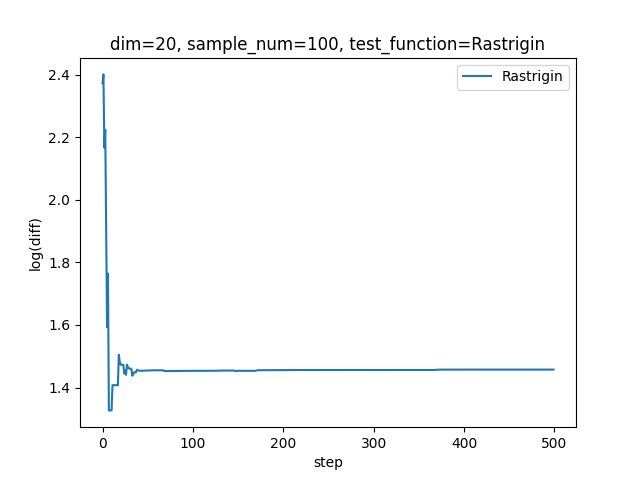
\includegraphics [width=10cm] {./result/Rastrigin_N_20.png}
                \end{figure}
        \end{itemize}
    \item Rosenbrock関数 \\
        関数の係数等は以下の設定で行った。
        \begin{equation}
            f(x) = \sum_{i=1}^{n-1} (100(x_{i+1} - x_i^2)^2 + (1 - x_i)^2),  (-5.00 \leq x_i \leq 10.00)
        \end{equation}
        この場合、最小値は全次元0のxを与えた際の0である。\\
        以下に、次元数とサンプル数を変化させた際の結果を示す。グラフは、各ステップにおける最適解との差の対数をプロットしたものである。
        \begin {itemize}
            \item 次元数: 2, サンプル数: 150, ステップ数: 500 \\
                この場合も、一度急速に最適値へと近づいたものの、再び誤差が大きくなってから収束したと思われる。各ステップでの変動幅が大きかったせいで最適値を通り越してしまって局所最小値に陥ったと思われる。 \\
                \begin{figure}[H]
                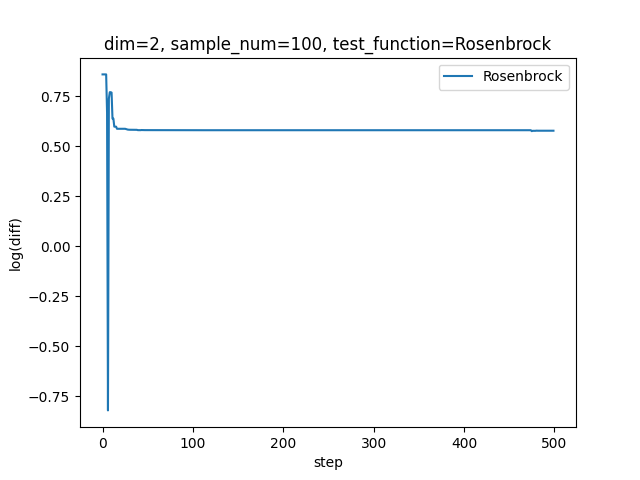
\includegraphics [width=10cm] {./result/Rosenbrock_N_2.png}
                \end{figure}
            \item 次元数: 20, サンプル数: 150, ステップ数: 500 \\
                数十ステップで収束したと思われる。誤差の大きさからすると、誤差が小さいわけではないので、局所最小値に陥った可能性がある。\\
                \begin{figure}[H]
                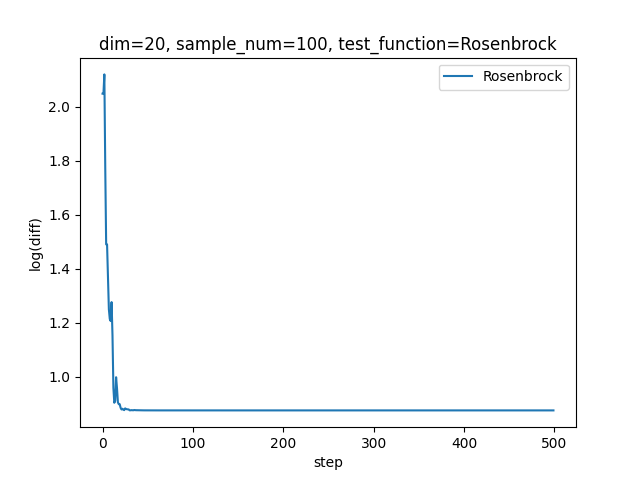
\includegraphics [width=10cm] {./result/Rosenbrock_N_20.png}
                \end{figure}
        \end{itemize}
    \item Griewank関数 \\
        関数の係数等は以下の設定で行った。
        \begin{equation}
            f(x) = \sum_{i=1}^{n} \frac{x_i^2}{4000} - \prod_{i=1}^{n} \cos(\frac{x_i}{\sqrt{i}}) + 1,  (-600.00 \leq x_i \leq 600.00)
        \end{equation}
        この場合、最小値は全次元0のxを与えた際の0である。\\
        以下に、次元数とサンプル数を変化させた際の結果を示す。グラフは、各ステップにおける最適解との差の対数をプロットしたものである。
        \begin {itemize}
            \item 次元数: 2, サンプル数: 12000, ステップ数: 500 \\
                100ステップを過ぎたあたりで収束していることが図から分かる。誤差もかなり小さいので、理想的に最適値を求められたと考えられる。\\
                \begin{figure}[H]
                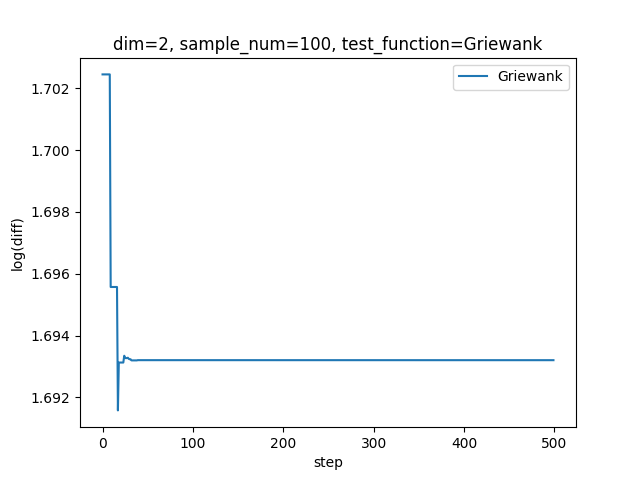
\includegraphics [width=10cm] {./result/Griewank_N_2.png}
                \end{figure}
            \item 次元数: 20, サンプル数: 12000, ステップ数: 500 \\
                50ステップを過ぎたあたりで収束していることが図から分かる。20次元とはいえ、誤差が小さいわけではないので、局所最小値に陥った可能性がある。\\
                \begin{figure}[H]
                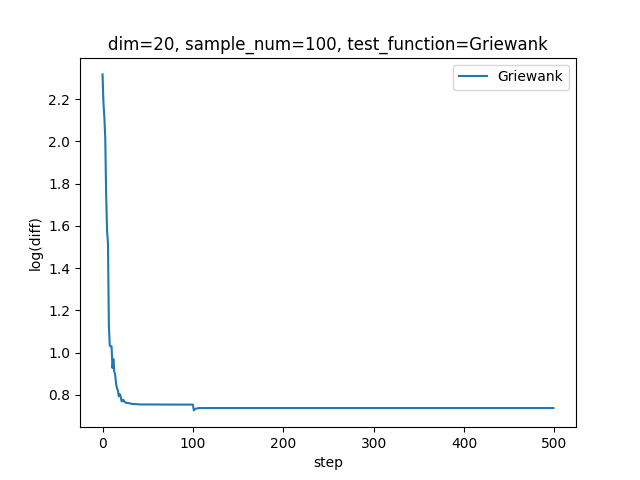
\includegraphics [width=10cm] {./result/Griewank_N_20.png}
                \end{figure}
        \end{itemize}
    \item Alpine関数 \\
        関数の係数等は以下の設定で行った。
        \begin{equation}
            f(x) = \sum_{i=1}^{n} |x_i \sin(x_i) + 0.1x_i|,  (-10.00 \leq x_i \leq 10.00)
        \end{equation}
        この場合、最小値は全次元0のxを与えた際の0である。\\
        以下に、次元数とサンプル数を変化させた際の結果を示す。グラフは、各ステップにおける最適解との差の対数をプロットしたものである。
        \begin {itemize}
            \item 次元数: 2, サンプル数: 200, ステップ数: 500 \\
                図から分かるようにステップを経るにつれて最適解との差の対数が単調にほぼ一様に小さくなっている。収束した様子は見られず、ステップ数を増加させれば収束した可能性がある。また、非常に最適値と近い値をとっていることがわかる。\\
                \begin{figure}[H]
                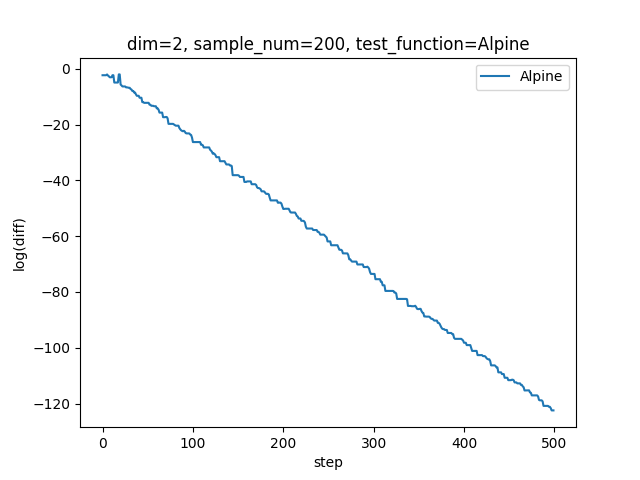
\includegraphics [width=10cm] {./result/Alpine_N_2.png}
                \end{figure}
            \item 次元数: 20, サンプル数: 200, ステップ数: 500 \\
                数十ステップで収束したと思われる。誤差の大きさからすると、20次元とはいえ、誤差が小さいわけではないので、局所最小値に陥った可能性がある。\\
                \begin{figure}[H]
                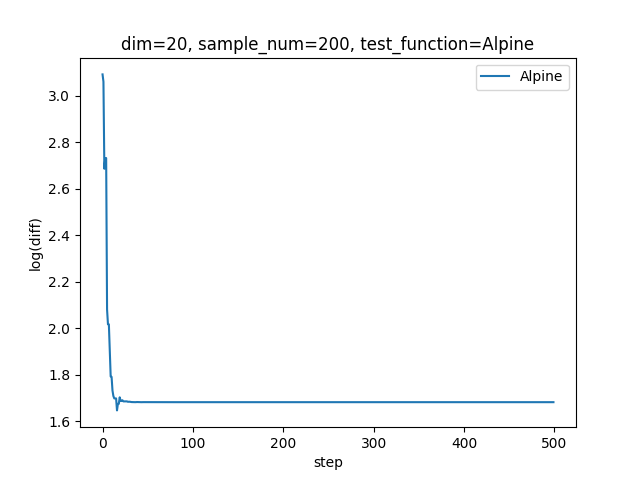
\includegraphics [width=10cm] {./result/Alpine_N_20.png}
                \end{figure}
        \end{itemize}
    \item 2n-minima関数 \\
        関数の係数等は以下の設定で行った。
        \begin{equation}
            f(x) = \sum_{i=1}^{n} (x_i^4 - 16x_i^2 + 5x_i),  (-5.00 \leq x_i \leq 5.00)
        \end{equation}
        この場合、最小値は全次元0のxを与えた際の0である。\\
        以下に、次元数とサンプル数を変化させた際の結果を示す。グラフは、各ステップにおける最適解との差の対数をプロットしたものである。
        \begin {itemize}
            \item 次元数: 2, サンプル数: 100, ステップ数: 500 \\
                一度急速に最適値へと近づいたものの、再び誤差が大きくなってから数十ステップで収束したと思われる。各ステップでの変動幅が大きかったせいで最適値を通り越してしまって局所最小値に陥ったと思われる。 \\
                \begin{figure}[H]
                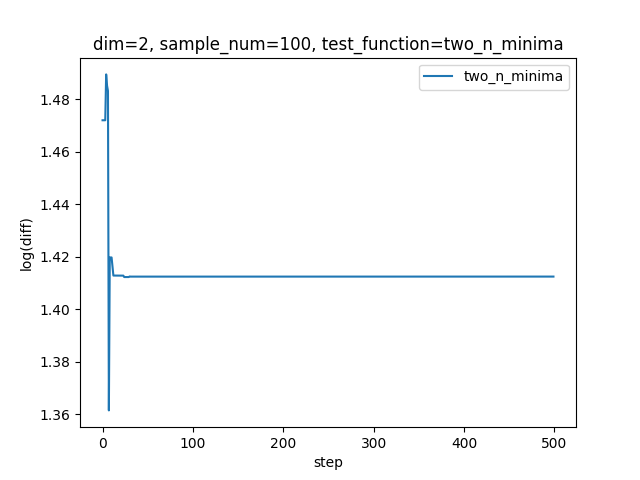
\includegraphics [width=10cm] {./result/two_n_minima_N_2.png}
                \end{figure}
            \item 次元数: 20, サンプル数: 100, ステップ数: 500 \\
                二度急速に最適値へと近づいたものの、その後は誤差が大きくなり続けて収束しないまま500ステップが終了している。ステップ数を増やしても局所最小値で収束する可能性はあるものの、最適値で収束する可能性は低いと考えられる。 \\
                \begin{figure}[H]
                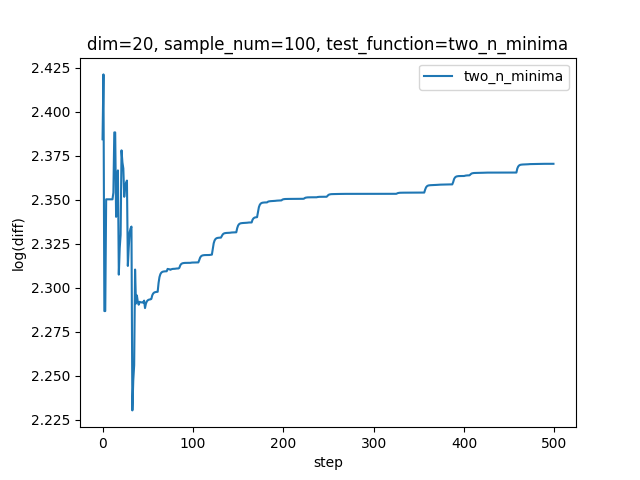
\includegraphics [width=10cm] {./result/two_n_minima_N_20.png}
                \end{figure}
        \end{itemize}
\end{enumerate}
\section{プログラムコード}
プログラムは、pso.py, test\_functions.py, main.pyの3つのファイルから構成される。pso.pyは、PSOのアルゴリズムを実装したものである。test\_functions.pyは、PSOの性能を評価するための関数を実装したものである。main.pyは、PSOの性能を評価するためのプログラムである。main.pyは、コマンドライン引数として、設定ファイルのパスを受け取る。設定ファイルは、yaml形式で記述されている。以下にはpythonのコードのみを示し、設定ファイルに関しては割愛する。\\
全てのコードは、\href{https://github.com/takeshiho0531/UTokyo-assignment/tree/8b08d135063f56aa030c3f327e3456ebad6ebe4a/3A/multi-agent_system/report1}{github}にて公開している。\\
\begin{lstlisting}[caption=pso.py]
    import random
    from typing import List
    
    import numpy as np
    
    
    def update_position(x: np.ndarray, v: np.ndarray) -> np.ndarray:
        updated_x = x + v
        return updated_x
    
    
    def update_velosity(
        x: np.ndarray,
        v: np.ndarray,
        personal_best_position: np.ndarray,
        global_best_position: np.ndarray,
        w=0.5,
        c1=0.14,
        c2=0.14,
    ) -> np.ndarray:
        r1 = random.uniform(0, 1)
        r2 = random.uniform(0, 1)
        updated_v = (
            w * v
            + c1 * r1 * (personal_best_position - x)
            + c2 * r2 * (global_best_position - x)
        )
        return updated_v
    
    
    def pso(
        step_num: int,
        initial: List[np.ndarray],  # 各要素にその点の全次元位置情報が含まれる
        criterion,
    ) -> dict:
        # initialize
        num = len(initial)
        position_list = initial
        velosity_list = np.zeros((len(initial), len(initial[0])))
        personal_best_position_list = list(position_list)
        personal_best_score_list = [criterion(p) for p in position_list]
        best_particle_idx = np.argmin(personal_best_score_list)
        global_best_position = personal_best_position_list[best_particle_idx]
    
        result = {}
    
        for t in range(step_num):
            for i in range(num):
                x = position_list[i]
                v = velosity_list[i]
                personal_best_position = personal_best_position_list[i]
    
                updated_x = update_position(x, v)
                position_list[i] = updated_x
    
                updated_v = update_velosity(
                    x, v, personal_best_position, global_best_position
                )
                velosity_list[i] = updated_v
    
                score = criterion(updated_x)
                if score < personal_best_score_list[i]:
                    personal_best_score_list[i] = score
                    personal_best_position_list[i] = updated_x
    
            best_particle_idx = np.argmin(personal_best_score_list)
            global_best_position = personal_best_position_list[best_particle_idx]
    
            result[t] = {
                "global_best_position": global_best_position,
                "global_best_score": min(personal_best_score_list),
            }
    
        return result
    
\end{lstlisting}
\newpage
\begin{lstlisting}[caption=test functions.py]
    import numpy as np


    def Sphere(x: np.ndarray) -> np.ndarray:
        return np.sum(x**2)
    
    
    def Rastrigin(x: np.ndarray) -> np.ndarray:
        return np.sum(x**2 - 10 * np.cos(2 * np.pi * x) + 10)
    
    
    def Rosenbrock(x: np.ndarray) -> np.ndarray:
        return np.sum(100 * (x[1:] - x[:-1] ** 2) ** 2 + (1 - x[:-1]) ** 2)
    
    
    def Griewank(x: np.ndarray) -> np.ndarray:
        return (
            np.sum(x**2 / 4000)
            - np.prod(np.cos(x / np.sqrt(np.arange(1, len(x) + 1))))
            + 1
        )
    
    
    def Alpine(x: np.ndarray) -> np.ndarray:
        return np.sum(np.abs(x * np.sin(x) + 0.1 * x))
    
    
    def two_n_minima(x: np.ndarray) -> np.ndarray:
        return np.sum(x**4 - 16 * x**2 + 5 * x)
\end{lstlisting}
\newpage
\begin{lstlisting}[caption=main.py]
    import sys

    import matplotlib.pyplot as plt
    import numpy as np
    import yaml
    from pso import pso
    from test_functions import Alpine, Griewank, Rastrigin, Rosenbrock, Sphere, two_n_minima
    
    
    def main(config_file_path: str):
        with open(config_file_path) as file:
            config = yaml.safe_load(file)
    
        dim = config["dim"]
        sample_num = config["sample_num"]
        low = config["low"]
        high = config["high"]
        step_num = config["step_num"]
    
        initial = []
        for i in range(sample_num):
            initial.append(np.random.uniform(low, high, dim))
    
        test_function = config["test_function"]
        if test_function == "Sphere":
            test_function = Sphere
        elif test_function == "Rastrigin":
            test_function = Rastrigin
        elif test_function == "Rosenbrock":
            test_function = Rosenbrock
        elif test_function == "Griewank":
            test_function = Griewank
        elif test_function == "Alpine":
            test_function = Alpine
        elif test_function == "two_n_minima":
            test_function = two_n_minima
        else:
            raise ValueError("test_function is invalid")
    
        ideal_position = np.zeros(dim)
    
        print(test_function.__name__)
        result = pso(step_num, initial, criterion=test_function)
        global_best_position_list = []
        diff_log_list = []
        for i in range(step_num):
            global_best_position_list.append(result[i]["global_best_position"])
            diff_log = np.log(np.linalg.norm(ideal_position - global_best_position_list[i]))
            diff_log_list.append(diff_log)
            print(f"step {i}: {diff_log}")
        plt.plot(diff_log_list, label=test_function.__name__)
        plt.xlabel("step")
        plt.ylabel("log(diff)")
        plt.title(
            f"dim={dim}, sample_num={sample_num}, test_function={test_function.__name__}"
        )
        plt.legend()
        plt.savefig(
            f"./result/{test_function.__name__}_N_{dim}.png"
        )
        print("--------------------")
    
    
    if __name__ == "__main__":
        main(sys.argv[1])
    
\end{lstlisting}


\end{document}